\documentclass[../main]{subfiles}
\begin{document}

\graphicspath{{../figures/chap1/}}

\section{本論文の構成}
\label{sec:configuration}
本論文は,全\ref{cp:conclusion}章から構成されている.
本論文の構成を\reffig{fig:configuration}に示す.

\refcp{cp:introduction}では,本研究の背景と先行研究,目的,対象としているシステムについて述べた.

\refcp{cp:estimation_theory}では,スペクトル画像からコーン指数を推定する原理について述べる.

\refcp{cp:proposed_method}では,提案手法について述べる.

\refcp{cp:verification_experiment}では,\refcp{cp:proposed_method}で述べた提案手法の有効性を確認するための検証実験とその結果,考察について述べる.

\refcp{cp:conclusion}では,本論文の結論と今後の展望を述べる.

\vspace{3\zh}
\begin{figure}[h]
    \centering
    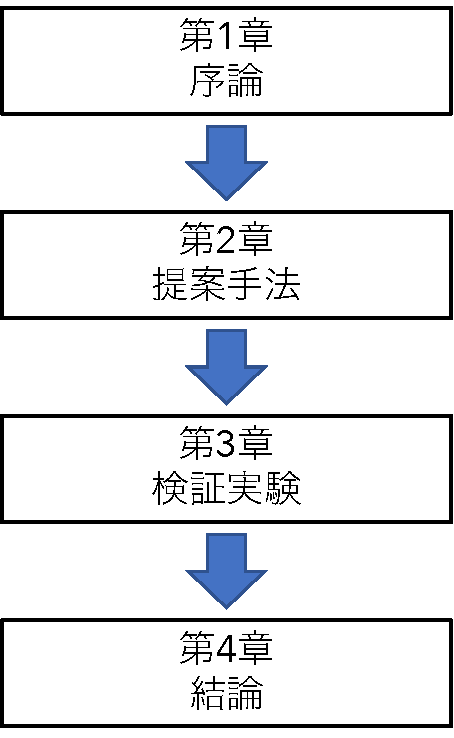
\includegraphics[keepaspectratio, width=0.35\linewidth]{configuration.pdf}
    \caption{本論文の構成}
    \label{fig:configuration}
\end{figure}

\end{document}